%!TEX root = ./main.tex

\section{O-RAN}

% SECTION TIMING: 52:00--69:00. Separate virtualization, disaggregation, openness, and control.

% TEACHING NOTE (2:00): Let students propose a deployment path before revealing the punchline.
\begin{frame}{Can base-station security become an app?}
  \ask{Who installs it? Who approves it? What happens at 2:00 a.m.?}

  \vspace{0.4em}
  \begin{center}
  \begin{tikzpicture}[node distance=0.32cm]
    \node[netnode,minimum width=2.0cm] (idea) {New defense};
    \node[netnode,minimum width=2.1cm,right=of idea] (vendor) {Vendor ticket};
    \node[netnode,minimum width=1.9cm,right=of vendor] (image) {New image};
    \node[corenode,minimum width=2.35cm,right=of image] (window) {Maintenance\\window};
    \draw[flow] (idea)--(vendor);
    \draw[flow] (vendor)--(image);
    \draw[flow] (image)--(window);
  \end{tikzpicture}
  \end{center}

  \takeaway{A programmable RAN asks: can a network behavior become a tested software application?}
\end{frame}

% TEACHING NOTE (2:00): This is a memory anchor, not evidence that every vendor cabinet looks identical.
\begin{frame}{A traditional RAN often arrived as a sealed appliance}
  \begin{columns}[T,onlytextwidth]
    \begin{column}{0.46\textwidth}
      \centering
      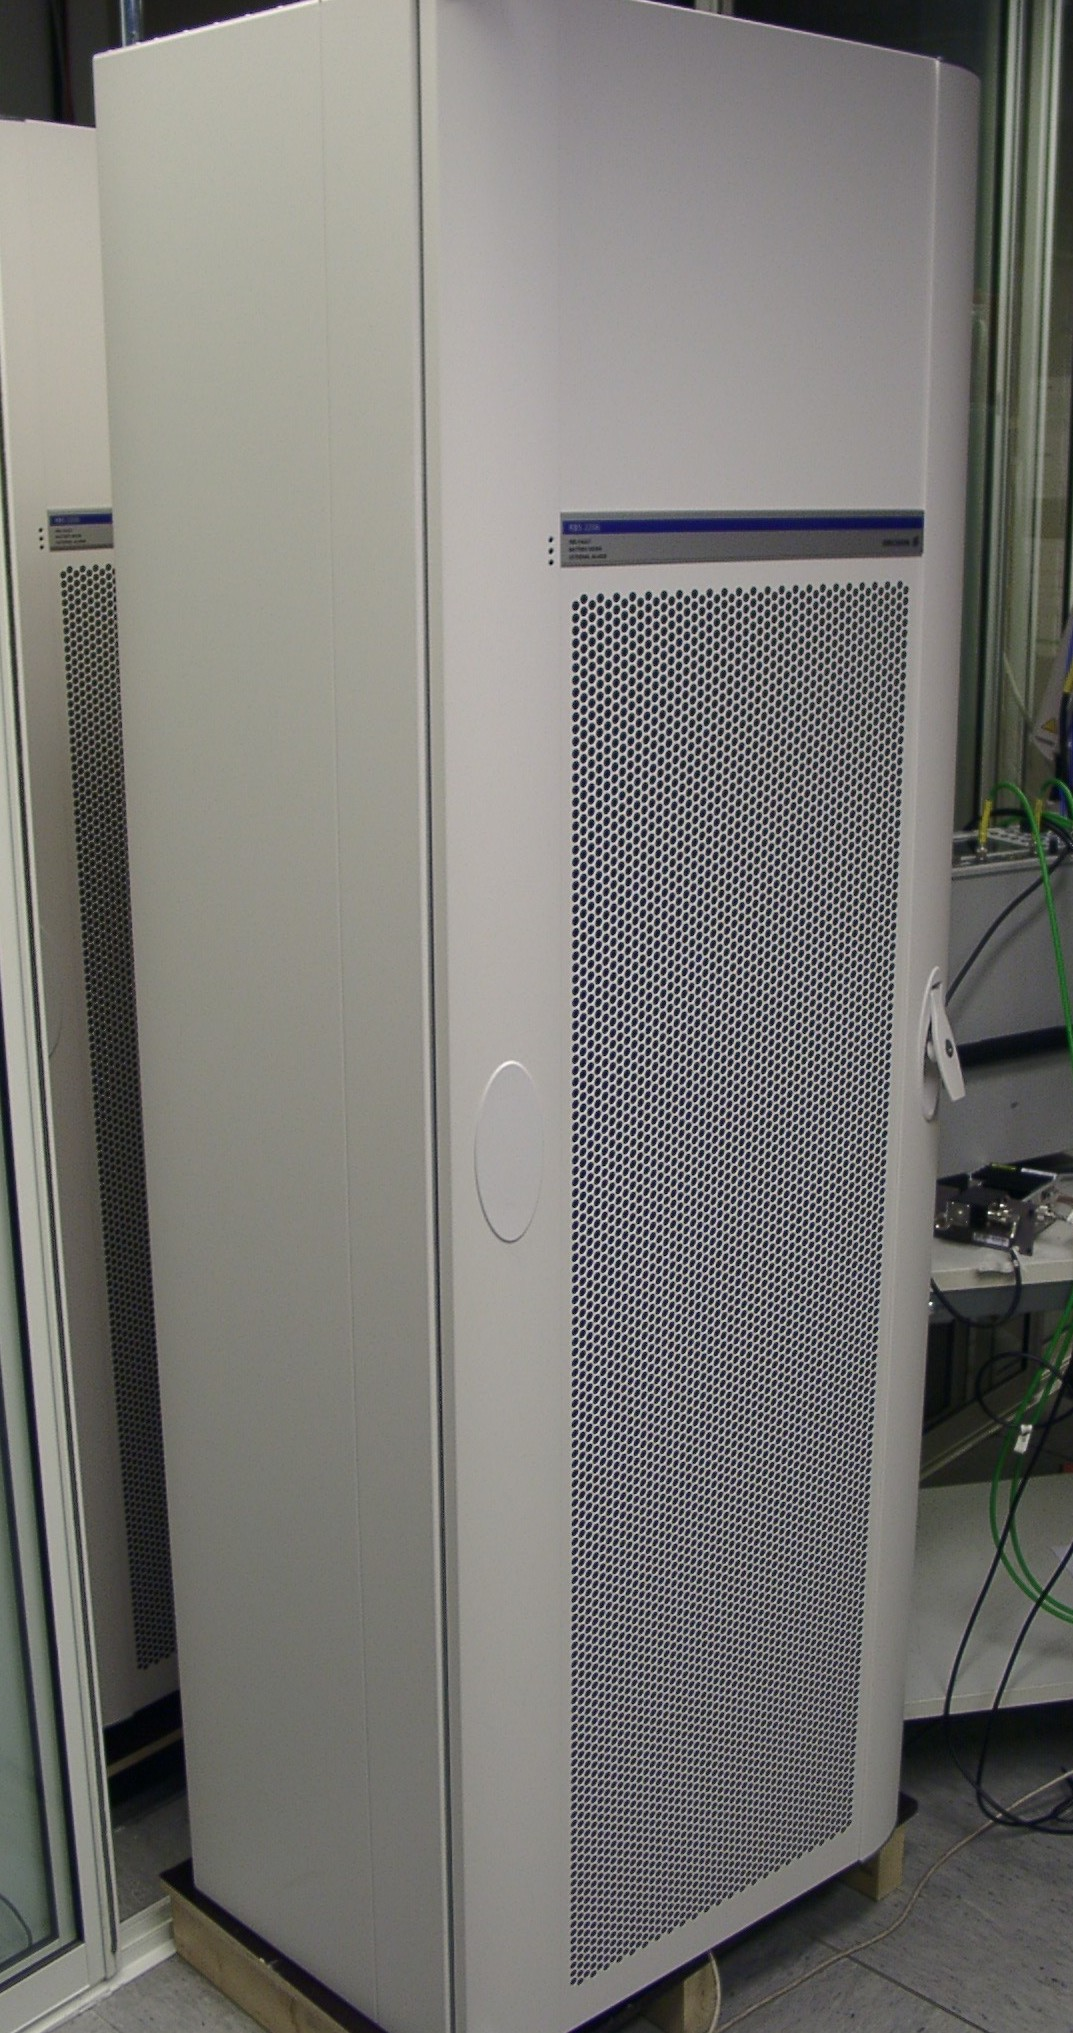
\includegraphics[height=0.67\textheight]{figure/ran_equipment_rack.jpg}
    \end{column}
    \begin{column}{0.51\textwidth}
      \vspace{0.8em}
      \begin{itemize}
        \item Hardware, software, and interfaces came as one system.
        \item One vendor owned most of the debugging story.
        \item Upgrades followed the vendor's release train.
      \end{itemize}

      \vspace{0.7em}
      \Large\centering
      Easy to blame one box.\\[0.3em]
      Hard to change one piece.
    \end{column}
  \end{columns}
  \source{https://commons.wikimedia.org/wiki/File:Telenor_base_station_radio_equipment_rack.jpg}{Telenor radio equipment rack}
\end{frame}

% TEACHING NOTE (2:30): Reveal one column at a time. Stress that these adjectives are not synonyms.
\begin{frame}{Four RAN models, four different questions}
  \centering
  \begin{tikzpicture}[node distance=0.22cm]
    \node[netnode,minimum width=2.18cm,minimum height=1.15cm] (d) {D-RAN\\[-1pt]{\scriptsize process at site}};
    \node[netnode,minimum width=2.18cm,minimum height=1.15cm,right=of d] (c) {C-RAN\\[-1pt]{\scriptsize pool baseband}};
    \node[netnode,minimum width=2.18cm,minimum height=1.15cm,right=of c] (v) {vRAN\\[-1pt]{\scriptsize software functions}};
    \node[oranode,minimum width=2.18cm,minimum height=1.15cm,right=of v] (o) {O-RAN\\[-1pt]{\scriptsize open + intelligent}};
    \draw[flow] (d)--(c); \draw[flow] (c)--(v); \draw[flow] (v)--(o);
  \end{tikzpicture}

  \vspace{0.8em}
  \begin{columns}[T,onlytextwidth]
    \begin{column}{0.32\textwidth}\centering
      \textbf{Virtualization}\\\small What runs where?
    \end{column}
    \begin{column}{0.32\textwidth}\centering
      \textbf{Disaggregation}\\\small Which functions split?
    \end{column}
    \begin{column}{0.32\textwidth}\centering
      \textbf{Open interfaces}\\\small Who can connect?
    \end{column}
  \end{columns}

  \vspace{0.7em}
  \takeaway{Cloud software does not automatically create an open, multi-vendor RAN.}
\end{frame}

% TEACHING NOTE (3:00): Zoom the lower RAN chain first, then the two RIC loops. Do not inventory every box.
\begin{frame}{O-RAN opens the seams---and adds control loops}
  \begin{columns}[T,onlytextwidth]
    \begin{column}{0.66\textwidth}
      \centering
      \begin{tikzpicture}[node distance=0.30cm,scale=0.84,transform shape]
        \node[oranode,minimum width=5.9cm,font=\small\bfseries] (smo) {SMO + Non-RT RIC};
        \node[oranode,minimum width=3.9cm,font=\small\bfseries,below=0.55cm of smo] (near) {Near-RT RIC};
        \node[oranode,minimum width=2.25cm,font=\scriptsize\bfseries,below left=0.65cm and -0.25cm of near] (cucp) {O-CU-CP};
        \node[oranode,minimum width=2.25cm,font=\scriptsize\bfseries,below right=0.65cm and -0.25cm of near] (cuup) {O-CU-UP};
        \node[netnode,minimum width=3.9cm,font=\small\bfseries,below=0.48cm of cucp.south east,anchor=north] (du) {O-DU};
        \node[netnode,minimum width=3.9cm,font=\small\bfseries,below=0.48cm of du] (ru) {O-RU};
        \draw[flow] (smo)--node[right,font=\tiny]{A1}(near);
        \draw[flow] (near)--node[left,font=\tiny]{E2}(cucp);
        \draw[flow] (near)--(cuup);
        \draw[flow] (cucp)--node[left,font=\tiny]{F1-C}(du);
        \draw[flow] (cuup)--node[right,font=\tiny]{F1-U}(du);
        \draw[flow] (du)--node[right,font=\tiny]{Open Fronthaul}(ru);
        \draw[flow,dashed] (smo.west) to[bend right=40] node[left,font=\tiny]{O1} (du.west);
      \end{tikzpicture}
    \end{column}
    \begin{column}{0.31\textwidth}
      \small
      \textbf{RAN chain}\\
      O-CU-CP / O-CU-UP\\
      O-DU / O-RU\\[0.7em]
      \textbf{Control}\\
      SMO + Non-RT RIC\\
      Near-RT RIC\\[0.7em]
      \textbf{Open seams}\\
      A1, E2, O1,\\Open Fronthaul
    \end{column}
  \end{columns}
  \source{https://mediastorage.o-ran.org/white-papers/O-RAN.WG1.Vertical-Industry-White-Paper-2023-12.pdf}{O-RAN ALLIANCE architecture, redrawn from 2023 white paper}
\end{frame}

% TEACHING NOTE (2:00): Ask for a show of hands before showing the right column.
\begin{frame}{Open RAN is not the same as open-source RAN}
  \begin{columns}[T,onlytextwidth]
    \begin{column}{0.47\textwidth}
      \begin{tcolorbox}[colback=blue!4,colframe=ranblue,title=Open RAN]
        Published interfaces\\[0.35em]
        Disaggregated functions\\[0.35em]
        Multi-vendor is \emph{possible}
      \end{tcolorbox}
    \end{column}
    \begin{column}{0.47\textwidth}
      \begin{tcolorbox}[colback=purple!5,colframe=ranpurple,title=Open source]
        Source code is available\\[0.35em]
        License permits reuse\\[0.35em]
        Interface may still be proprietary
      \end{tcolorbox}
    \end{column}
  \end{columns}

  \vspace{0.55em}
  \ask{If two boxes claim the same interface, will they work when plugged together?}
  \takeaway{A specification begins interoperability; profiles, testing, and integration finish it.}
  \source{https://www.o-ran.org/o-ran-resources}{O-RAN ALLIANCE architecture and resources}
\end{frame}

% TEACHING NOTE (3:00): Video 0:18--1:12. Offline fallback: use the diagram and traffic-steering example.
\begin{frame}{RIC makes optimization an application}
  \begin{columns}[T,onlytextwidth]
    \begin{column}{0.45\textwidth}
      \href{https://www.youtube.com/watch?v=dgiWoTrQ19I}{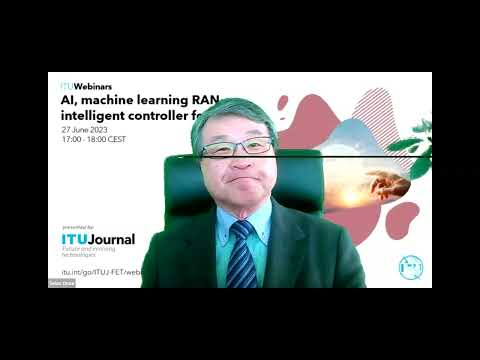
\includegraphics[width=\linewidth]{figure/oran_ric_video.jpg}}
      \centering\small\textcolor{blue}{\underline{Play: a real RIC demo (0:18--1:12)}}
    \end{column}
    \begin{column}{0.52\textwidth}
      \begin{tikzpicture}[node distance=0.48cm]
        \node[oranode,minimum width=4.6cm] (nonrt) {Non-RT RIC + rApp\\[-1pt]{\scriptsize policy, models, longer horizon}};
        \node[oranode,minimum width=4.6cm,below=of nonrt] (near) {Near-RT RIC + xApp\\[-1pt]{\scriptsize faster decisions: roughly 10 ms--1 s}};
        \node[netnode,minimum width=4.6cm,below=of near] (ran) {O-CU / O-DU / O-RU};
        \draw[flow] (nonrt)--node[right]{\scriptsize A1}(near);
        \draw[flow] (near)--node[right]{\scriptsize E2}(ran);
      \end{tikzpicture}

      \small\textbf{Example: traffic steering}\\
      rApp sets policy; xApp reacts to load; RAN executes.
    \end{column}
  \end{columns}
  \source{https://www.youtube.com/watch?v=dgiWoTrQ19I}{ITU, O-RAN / RIC demonstration}
\end{frame}

% TEACHING NOTE (2:30): End with the tradeoff question; accept multiple defensible answers.
\begin{frame}{Opening the RAN creates both options and work}
  \begin{columns}[T,onlytextwidth]
    \begin{column}{0.47\textwidth}
      \begin{tcolorbox}[colback=green!5,colframe=softgreen,title=Options]
        \begin{itemize}
          \item More vendor choice
          \item Faster software experiments
          \item Programmable optimization
        \end{itemize}
      \end{tcolorbox}
    \end{column}
    \begin{column}{0.47\textwidth}
      \begin{tcolorbox}[colback=orange!6,colframe=coreorange,title=Work]
        \begin{itemize}
          \item Fronthaul and timing
          \item Integration and testing
          \item Larger security surface
        \end{itemize}
      \end{tcolorbox}
    \end{column}
  \end{columns}

  \vspace{0.05em}
  \ask{Would you rather debug one black box or five open interfaces?}
  \takeaway{Openness moves work. It does not make the work disappear.}
  \source{https://mediastorage.o-ran.org/overview/o-ran-overview-presentation/o-ran-overview-of-the-o-ran-alliance-presentation.pdf}{O-RAN ALLIANCE overview (2026)}
\end{frame}
